%\usepackage{subfig}

\chapter{Observational Procedures}

the full description of the survey is in: D. J. Sand et. al. 2011

MegaCam wide field imager on the CFHT (Canada-France-Hawii Telescope). The cluster sample consisted of 101 clusters within the range of redshifts from 0.05 < z< 0.55

58 clusters from the MENEACs (Multi-Epoch nearby cluster survey)

The meneacs clusters represent all clusters in the BAX X-ray cluster database that are observable fof the CFHT

the redshifts of the clusters as given by C. Bildfell et. al. 2012 

G, U, I and R images


\begin{table}[]
\centering

\begin{tabular}{ccccc}
Cluster & $z$   & $\sigma(km/s)$ & $d(Mpc)$ & $\theta_{E}(")$ \\ \hline \hline
A1033   & 0.126 & 762            &  & 14.6155  \\
*A1068  & 0.138 & 740            &  & 13.5945  \\
A1132   & 0.136 & 727            &  & 13.1515   \\
*A119   & 0.044 & 875            &  & 21.0798   \\
*A1413  & 0.143 & 881            &  & 19.1569   \\
A1650   & 0.084 & 720            &  & 13.6758   \\
A1651   & 0.085 & 903            &  & 21.4876   \\
A1795   & 0.062 & 778            &  & 16.3514   \\
*A2029  & 0.077 & 1152           &  & 35.2776   \\
A2050   & 0.118 & 854            &  & 18.5258   \\
A2055   & 0.102 & 697            &  & 12.5642   \\
A2064   & 0.108 & 675            &  & 11.7048   \\
*A2065  & 0.073 & 1095           &  & 32.0110   \\
A2069   & 0.116 & 966            &  & 23.7574   \\
*A2142  & 0.091 & 1086           &  & 30.8756   \\
*A2319  & 0.056 & 1101           &  & 32.9563   \\
A2420   & 0.085 & ~800           &  & 16.8653   \\
A2440   & 0.091 & 766            &  & 15.3608   \\
A2597   & 0.085 & 682            &  & 12.2569   \\
A2627   & 0.126 & ~800           &  & 16.1096   \\
A2703   & 0.114 & ~800           &  & 16.3307   \\
A399    & 0.072 & ~800           &  & 17.1049   \\
A553    & 0.066 & ~800           &  & 17.2155   \\
*A655   & 0.127 & ~800           &  & 16.0911   \\
*A754   & 0.054 & ~800           &  & 17.4367   \\
A763    & 0.085 & ~800           &  & 16.8653   \\
A795    & 0.136 & ~800           &  & 15.9252   \\
*A85    & 0.055 & ~800           &  & 17.4182   \\
A961    & 0.124 & ~800           &  & 16.1464   \\
A990    & 0.144 & ~800           &  & 15.7778   
\end{tabular}
\caption{My caption}
\label{my-label}
\end{table}

\section{Sextractor}

Stars and selection of galaxies

\section{Galfit}

 The parameters C0, B1, B2, F1, F2, etc. listed below are hidden 
 from the user unless he/she explicitly requests them.  These can  be tagged on to the end of any previous components except, of 
 course, the PSF and the sky -- although galfit won't bar you from doing 
 so, and will just ignore them.  Note that a Fourier or Bending mode 
 amplitude of exactly 0 will cause GALFIT to crash because the 
 derivative image GALFIT computes internally will be entirely 0.  If a 
 Fourier or Bending amplitude is set to 0 initially GALFIT will reset it  
 to a value of 0.01.  To prevent GALFIT from doing so, one can set it to any 
 other value.

  Bending modes
B1)  0.07      1        Bending mode 1 (shear)
B2)  0.01      1        Bending mode 2 (banana shape)
B3)  0.03      1        Bending mode 3 (S-shape)

  Azimuthal fourier modes
F1)  0.07  30.1  1  1   Az. Fourier mode 1, amplitude and phase angle
F2)  0.01  10.5  1  1   Az. Fourier mode 2, amplitude and phase angle
F6)  0.03  10.5  1  1  Az. Fourier mode 6, amplitude and phase angle
F10)  0.08  20.5  1  1   Az. Fourier mode 10, amplitude and phase angle
F20)  0.01  23.5  1  1   Az. Fourier mode 20, amplitude and phase angle

  Traditional Diskyness/Boxyness parameter c
C0) 0.1         0       traditional diskyness(-)/boxyness(+)

\section{Color images}


In er.  

\begin{figure}[H]
\centering
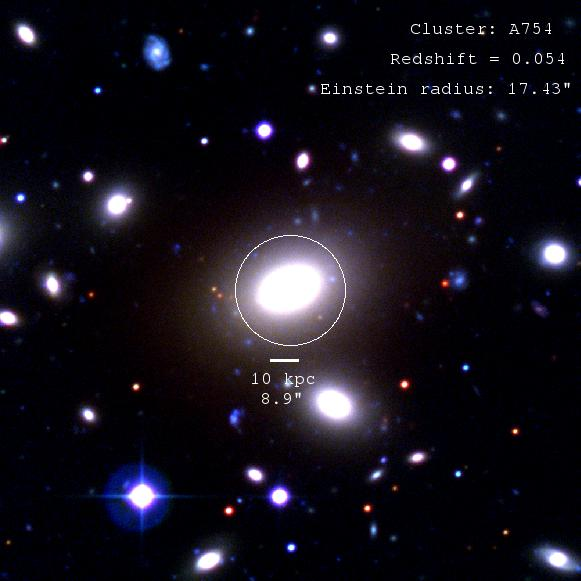
\includegraphics[width=12cm]{images/cA754.jpg}
\caption[M]{G}
\end{figure}

\begin{figure}[H]
\centering
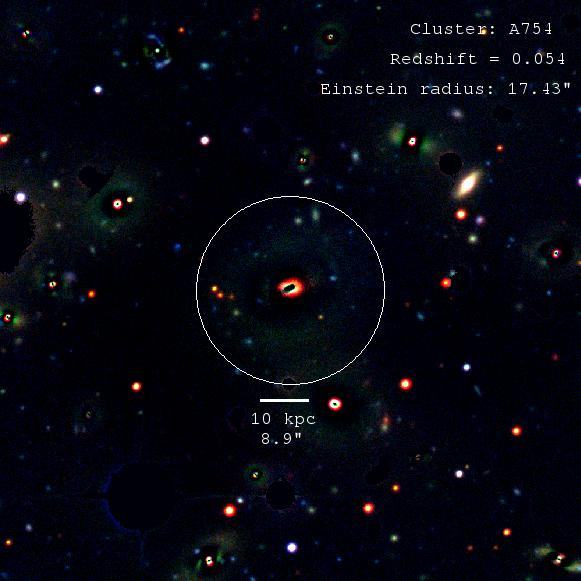
\includegraphics[width=12cm]{images/cA754_galfit.jpg}
\caption[M]{G}
\end{figure}


\section{Photometric Redshift}

(using as reference Benitez, Narciso 2000)